% A schematic diagram showing the shape of the feature map as it passes through the network.

% In the encoding path, the feature map is transformed with two successive 3x3x3 convolutions and ReLU activations
% followed by a 2x2x2 max-pooling operation that reduces the spatial dimensions by half.

% In the decoding path, information from fine and coarse scales is combined through skip connections.
% The feature map is upsampled by a factor of 2 using a 3x3x3 transposed convolution.
% This is combined with the feature map from the contracting path through a skip connection,
% which is passed through an attention gate before being concatenated with the upsampled feature map.
% The feature map from deeper in the network acts as the attention gating signal.
% The upsampled feature map and attended feature map from the skip connection are concatenated and
% convolved along the channel dimension to produce the final feature map.

\documentclass{standalone}
\usepackage{tikz}
\usetikzlibrary{shapes.geometric, arrows.meta, positioning}

\newlength{\blockwidth}
\setlength{\blockwidth}{3cm}

\newlength{\yshift}
\setlength{\yshift}{-0.5cm}
\newlength{\xshift}
\setlength{\xshift}{0.5cm}

\tikzstyle{block} = [rectangle, draw, text centered, text width=\blockwidth, minimum height=0.333* \blockwidth]
\tikzstyle{arrow} = [thick,->,>=stealth]
\tikzstyle{skip} = [thick, dashed,->,>=stealth]
\tikzstyle{attention} = [circle, draw, text centered, minimum height=1cm, minimum width=2em]

\begin{document}
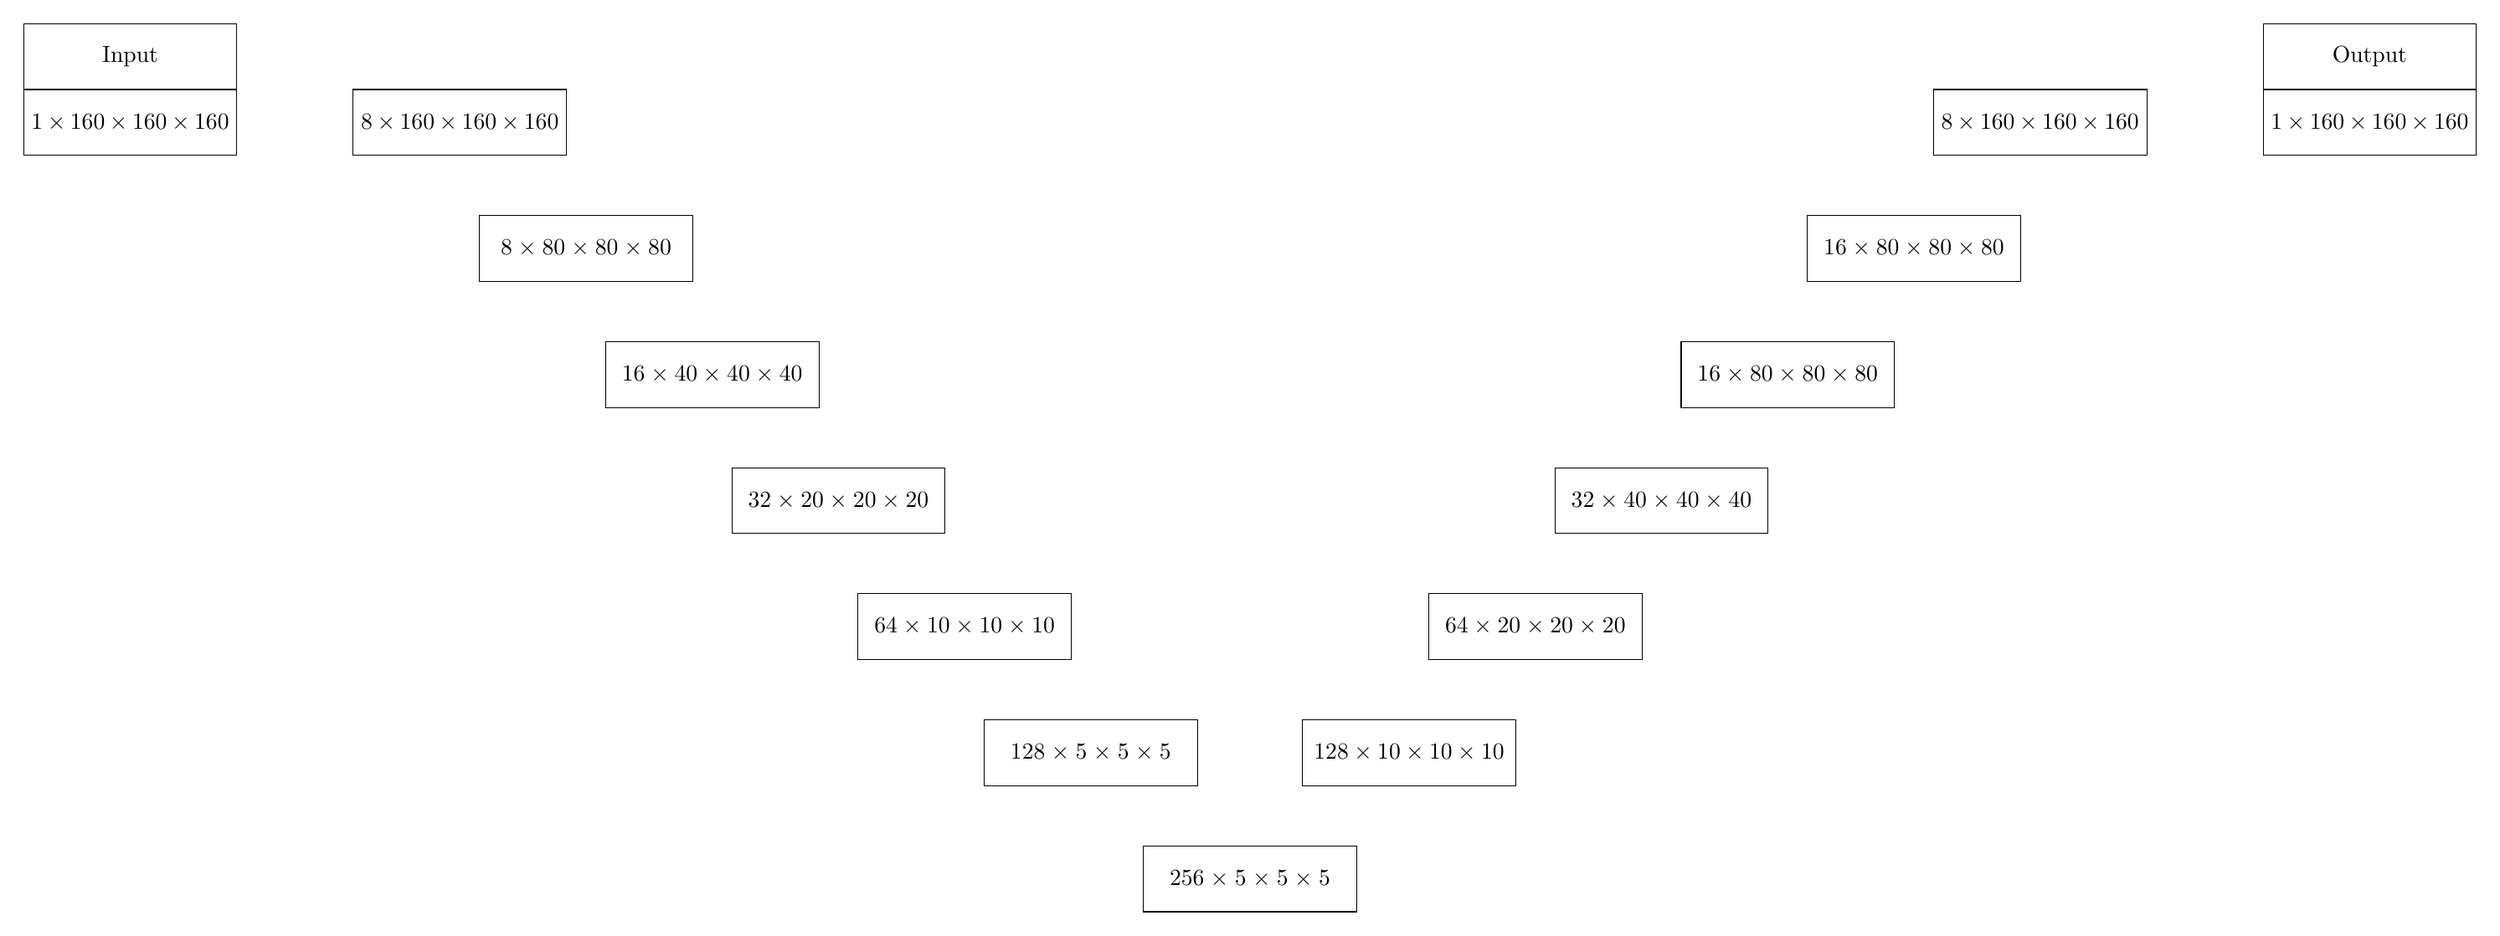
\begin{tikzpicture}[node distance=2cm]

    % Input
    \node (input_label) [block] {Input};
    \node (input) [block, below of=input_label, yshift=1cm]{$1\times160\times160\times160$};

    % Contracting path
    \node (head) [block, right of=input, xshift=\blockwidth] {$8\times160\times160\times160$};

    \node (enc1) [block, below right of=head, yshift=\yshift, xshift=\xshift]{$8\times80\times80\times80$};
    \node (enc2) [block, below right of=enc1, yshift=\yshift, xshift=\xshift]{$16\times40\times40\times40$};
    \node (enc3) [block, below right of=enc2, yshift=\yshift, xshift=\xshift]{$32\times20\times20\times20$};
    \node (enc4) [block, below right of=enc3, yshift=\yshift, xshift=\xshift]{$64\times10\times10\times10$};
    \node (enc5) [block, below right of=enc4, yshift=\yshift, xshift=\xshift]{$128\times5\times5\times5$};

    % Bottom layer
    \node (bottom) [block, below right of=enc5, yshift=\yshift, xshift=2\xshift]{$256\times5\times5\times5$};

    % Expanding Path
    \node (dec5) [block, above right of=bottom, yshift=-\yshift, xshift=2\xshift]{$128\times10\times10\times10$};
    \node (dec4) [block, above right of=dec5, yshift=-\yshift, xshift=\xshift]{$64\times20\times20\times20$};
    \node (dec3) [block, above right of=dec4, yshift=-\yshift, xshift=\xshift]{$32\times40\times40\times40$};
    \node (dec2) [block, above right of=dec3, yshift=-\yshift, xshift=\xshift]{$16\times80\times80\times80$};
    \node (dec1) [block, above right of=dec2, yshift=-\yshift, xshift=\xshift]{$16\times80\times80\times80$};

    \node (reduce) [block, above right of=dec1, yshift=-\yshift, xshift=\xshift]{$8\times160\times160\times160$};

    % Output
    \node (output) [block, right of=reduce, xshift=\blockwidth] {$1\times160\times160\times160$};
    \node (output_label) [block, above of=output, yshift=-1cm]{Output};

    % % Attention Mechanisms
    % \node (att5) [attention, above right of=bottom, xshift=-1.5cm, yshift=1.5cm] {Att};
    % \node (att4) [attention, above right of=dec5, xshift=-1.5cm, yshift=1.5cm] {Att};
    % \node (att3) [attention, above right of=dec4, xshift=-1.5cm, yshift=1.5cm] {Att};
    % \node (att2) [attention, above right of=dec3, xshift=-1.5cm, yshift=1.5cm] {Att};
    % \node (att1) [attention, above right of=dec2, xshift=-1.5cm, yshift=1.5cm] {Att};

    % ==== Arrows
    % Contracting
    % \draw [arrow] (input) -- (head);
    % \draw [arrow] (head_size) -- (enc1_size);
    % \draw [arrow] (enc1_size) -- (enc2_size);
    % \draw [arrow] (enc2_size) -- (enc3_size);
    % \draw [arrow] (enc3_size) -- (enc4_size);
    % \draw [arrow] (enc4_size) -- (enc5_size);
    % \draw [arrow] (enc5_size) -- (bottom);

    % % Expanding
    % \draw [arrow] (bottom) -- (dec5);
    % \draw [arrow] (dec5) -- (dec4);
    % \draw [arrow] (dec4) -- (dec3);
    % \draw [arrow] (dec3) -- (dec2);
    % \draw [arrow] (dec2) -- (dec1);
    % \draw [arrow] (dec1) -- (reduce);
    % \draw [arrow] (reduce) -- (output);

    % % Attention
    % \draw [skip] (bottom) -- (att5);
    % \draw [skip] (dec5) -- (att4);
    % \draw [skip] (dec4) -- (att3);
    % \draw [skip] (dec3) -- (att2);
    % \draw [skip] (dec2) -- (att1);

    % % Skip Connections
    % \draw [skip] (enc5) -- (att5);
    % \draw [skip] (att5) -- (dec5);
    % \draw [skip] (enc4) -- (att4);
    % \draw [skip] (att4) -- (dec4);
    % \draw [skip] (enc3) -- (att3);
    % \draw [skip] (att3) -- (dec3);
    % \draw [skip] (enc2) -- (att2);
    % \draw [skip] (att2) -- (dec2);
    % \draw [skip] (enc1) -- (att1);
    % \draw [skip] (att1) -- (dec1);

\end{tikzpicture}
\end{document}
